\documentclass{beamer}
\usecolortheme{whale}

% Loading packages
\usepackage[utf8]{inputenc}
\usepackage{tcolorbox}
\usepackage{amsmath}
\usepackage[T1]{fontenc}
\usepackage{lmodern}
\usepackage{graphicx,float,subcaption,geometry,booktabs, multicol}
\usepackage[linesnumbered,ruled]{algorithm2e}

% Define details on slide cover page
\title{Recurrent Auto-Encoder Model for\\ Large-Scale Industrial Sensor Signal Analysis}
\author{Timothy Wong \inst{1,2} \and Zhiyuan Luo \inst{1}}
\institute{Royal Holloway, University of London, \\Egham TW20 0EX, \\United Kingdom.}

\institute{
\inst{1} Royal Holloway, University of London, Egham TW20 0EX. \and
\inst{2} Centrica plc, Millstream, Maindenhead Road, Windsor SL4 5GD.}
                      
\date{
{19\textsuperscript{th} International Conference on\\
Engineering Applications of Neural Networks (EANN 2018)\\
3-5 September 2018 - Bristol, UK}
}

% Begins the slide deck
\begin{document}

\section{Cover}
\begin{frame}
\maketitle
\end{frame}

\section{Background}

\begin{frame}[shrink]{Background}
  \begin{itemize}
    \item Gas compression sub-system at a gas terminal 
    \begin{itemize}
      \item Two centrifugal compressors driven on a single shaft
      \item Powered by aeroderivative gas turbine
      \item Regulates gas pressure at a certain level
    \end{itemize}
    \begin{figure}
    	\centering
    	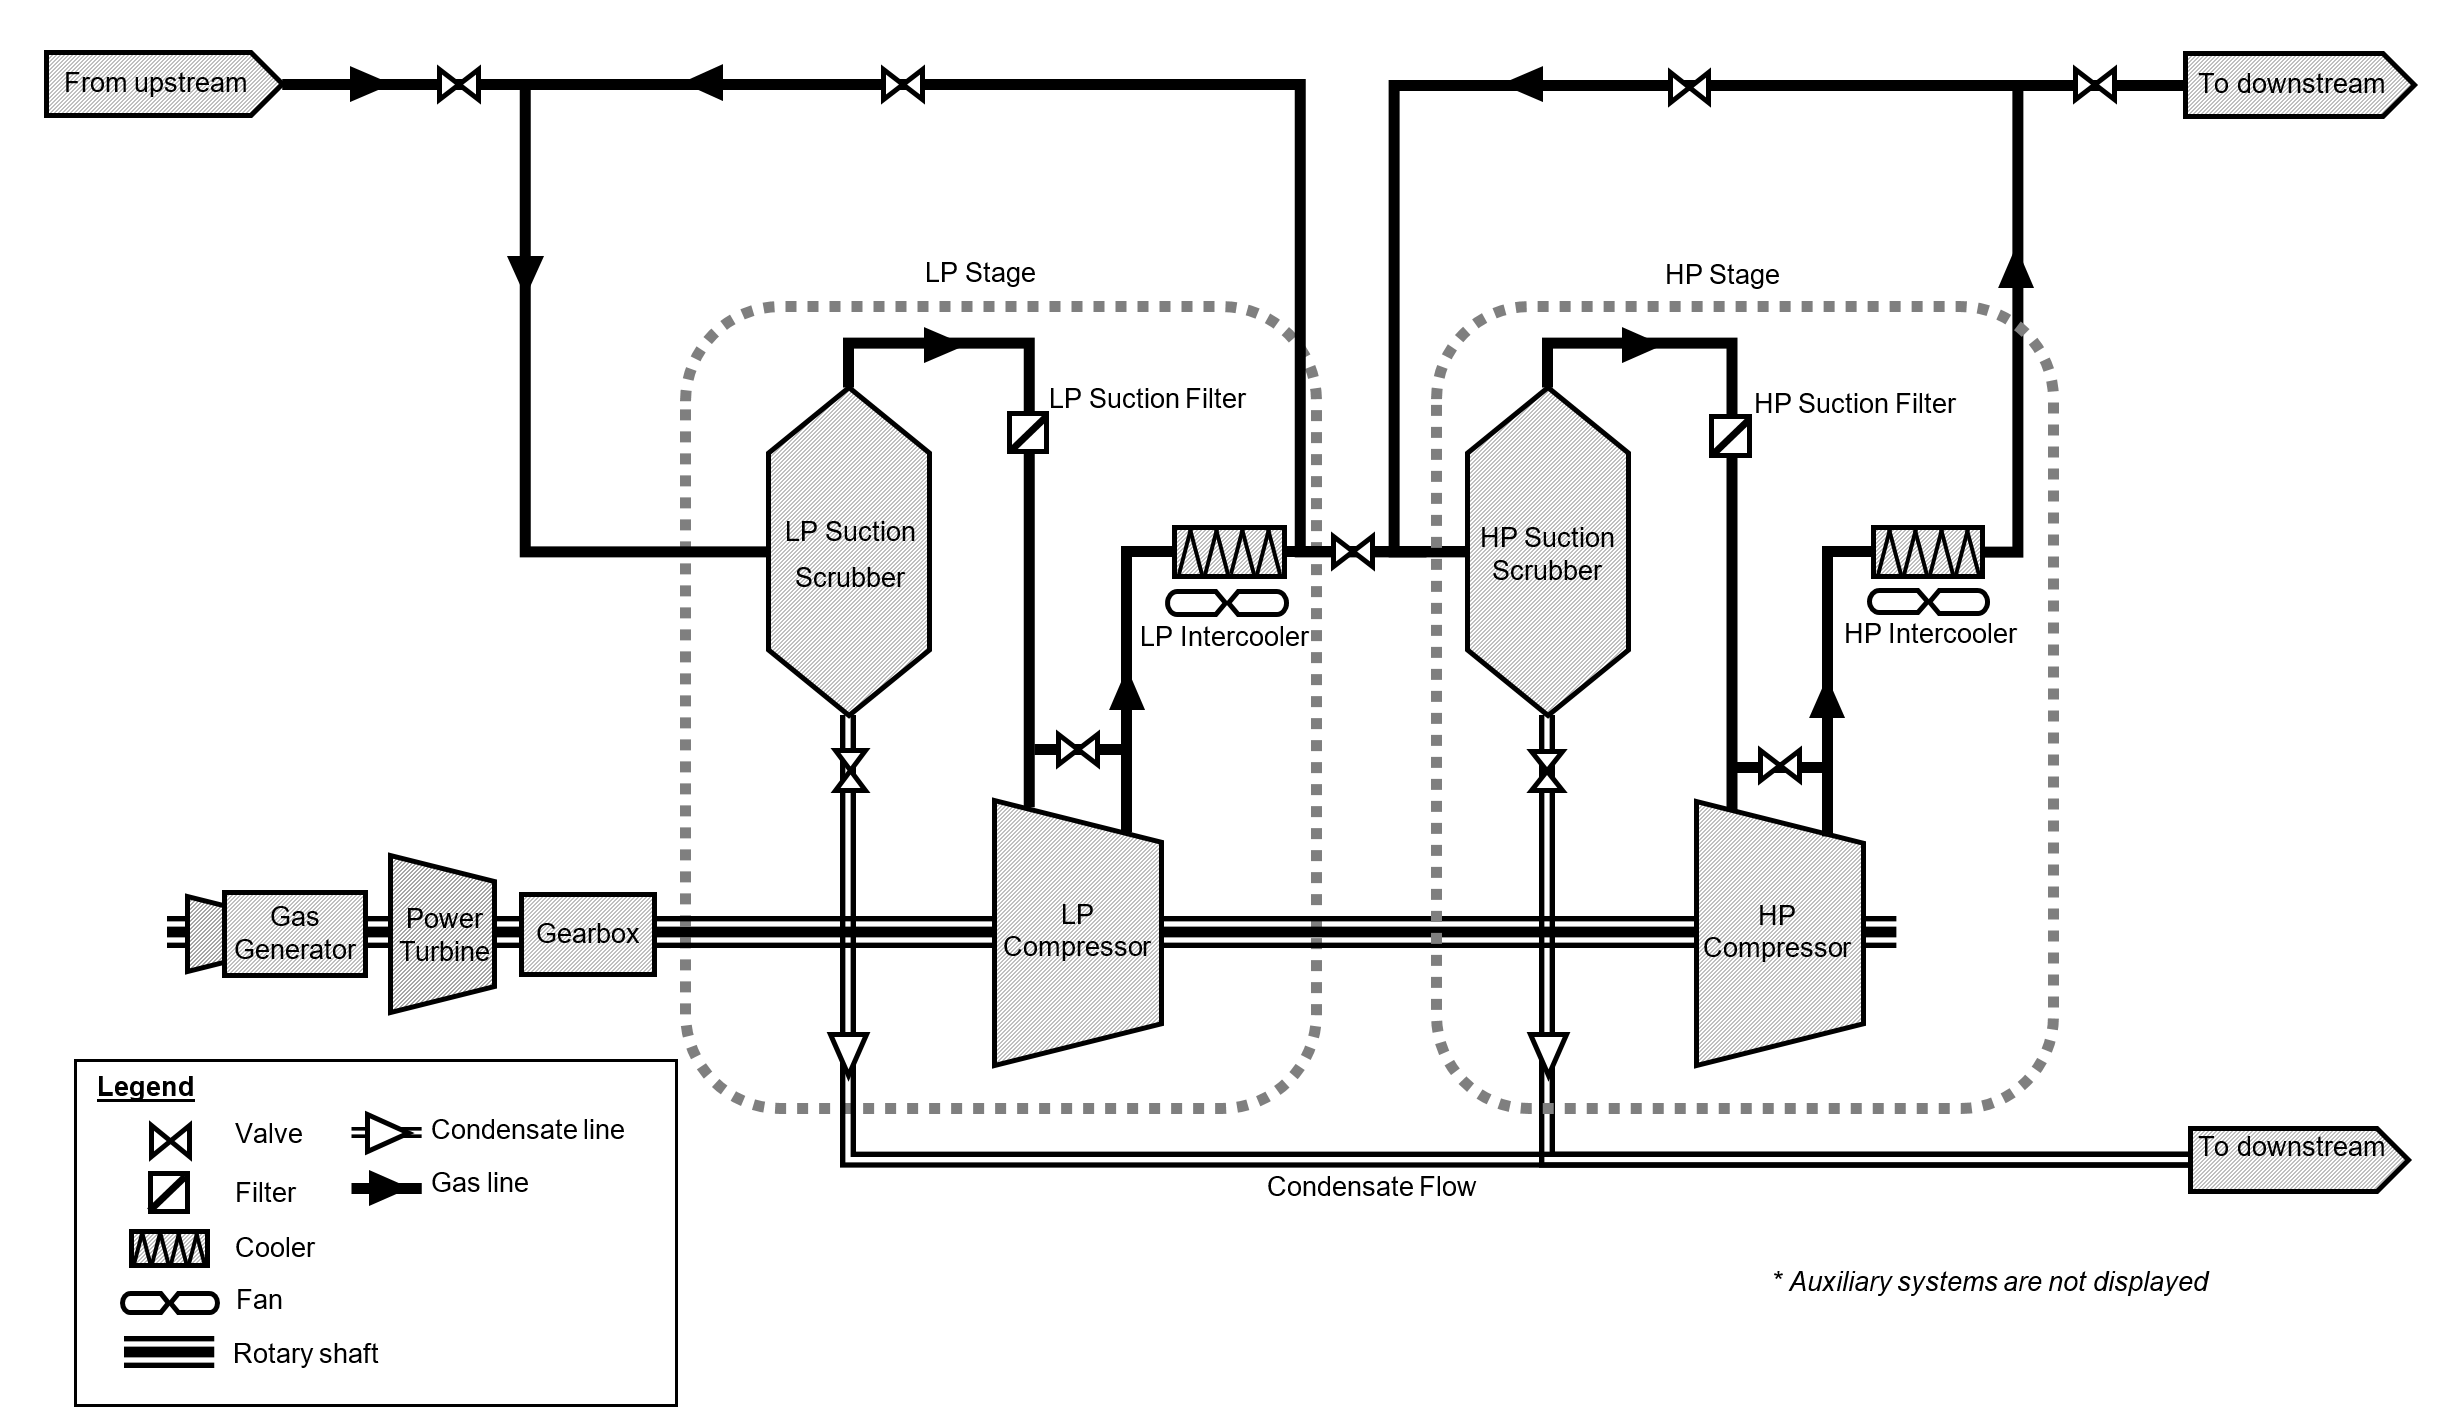
\includegraphics[width=1\textwidth]{process_diagram.png}
      \caption{Simplified process diagram for the compression sub-system}
    \end{figure}
  \end{itemize}
\end{frame}

\begin{frame}{Components}
  \begin{figure}
    \centering
    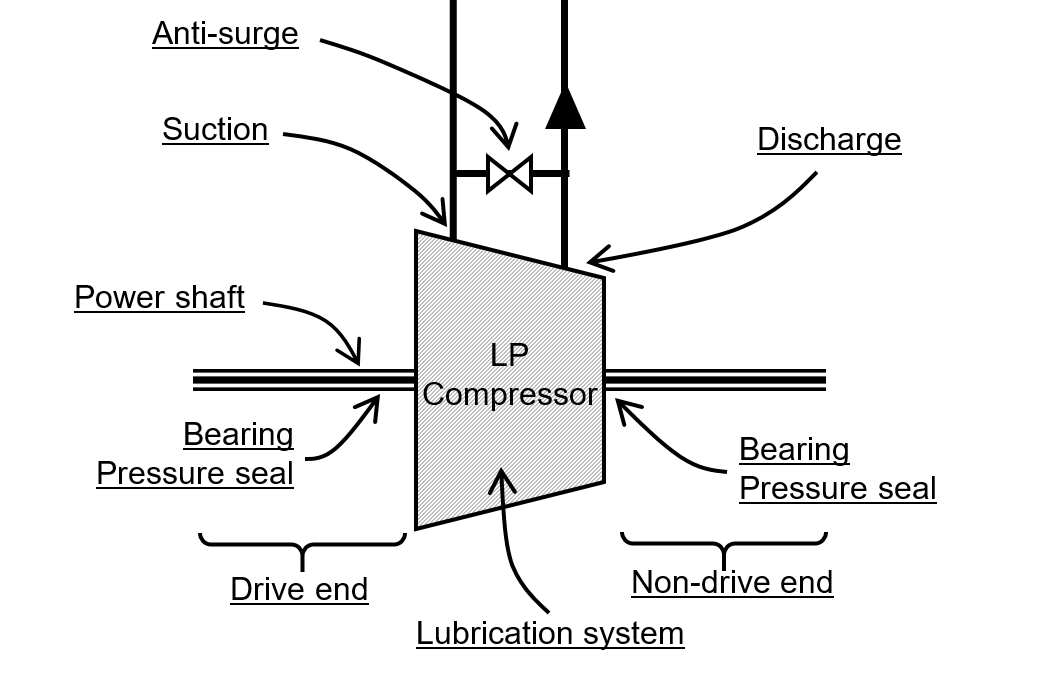
\includegraphics[width=0.8\textwidth]{lp-stage.PNG}
    \caption{Centrifugal compressor (LP stage)}
  \end{figure}
\end{frame}

\begin{frame}{Components}
  \begin{figure}
    \centering
    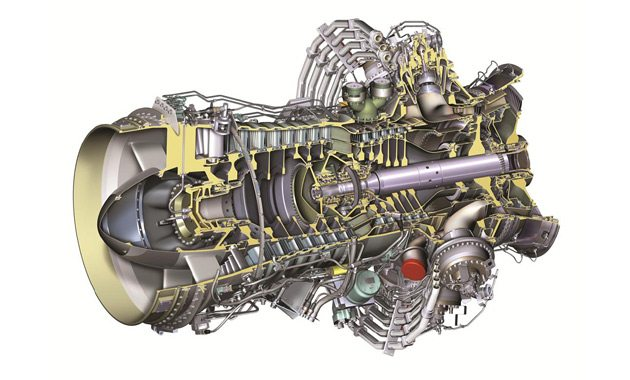
\includegraphics[width=0.47\textwidth]{rb211.jpg}
    \hfill
    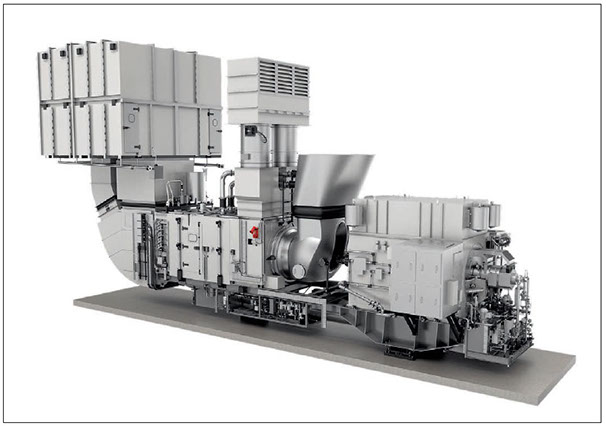
\includegraphics[width=0.47\textwidth]{rb211_package.jpg}
    \caption{Jet engine package}
  \end{figure}
\end{frame}



\begin{frame}{Problem}
  \begin{itemize}
    \item Large-scale industrial processes contains many sensors
    \item Sensor records continuous stream of real-valued measurements \\
          (e.g. temperature, pressure, rotary speed… etc.)
  \end{itemize}
  \begin{tcolorbox}[title=Research Question]
    Can we determine the underlying operating states of the process?
  \end{tcolorbox}
\end{frame}

\section{Method}

\begin{frame}{Data Preprocessing}
  \begin{itemize}
    \item Unevenly-spaced time series (inconsistent interval)
    \item Can be convert into regularly-spaced time series through downsampling.
    \item \(P\) sensors can form a \(P\)-dimensional multivariate time series.
    \[ \{ \mathbb{R}_t^P:t\in [1,T] \} \]
  \end{itemize}
\end{frame}


\begin{frame}[shrink]{Recurrent Auto-Encoder Model}
  \begin{itemize}
    \item RNN Encoder-decoder model
    \item Convert to recurrent auto-encoder by aligning input/output time steps
    \item Performs partial reconstruction on the decoder side
    \item Decoder dimension smaller than Encoder dimension
    \item Deep structure learns abstract temporal patterns
  \end{itemize}
  \[
    \begin{cases} 
      f_{encoder} : \{ \mathbb{R}_t^P:t \in [1, T] \} \rightarrow c \\
      f_{decoder} : c \rightarrow \{ \mathbb{R}_t^K:t \in [1, T] \} \\
    \end{cases} K \leqslant P
  \]
  \begin{figure}
    \centering
    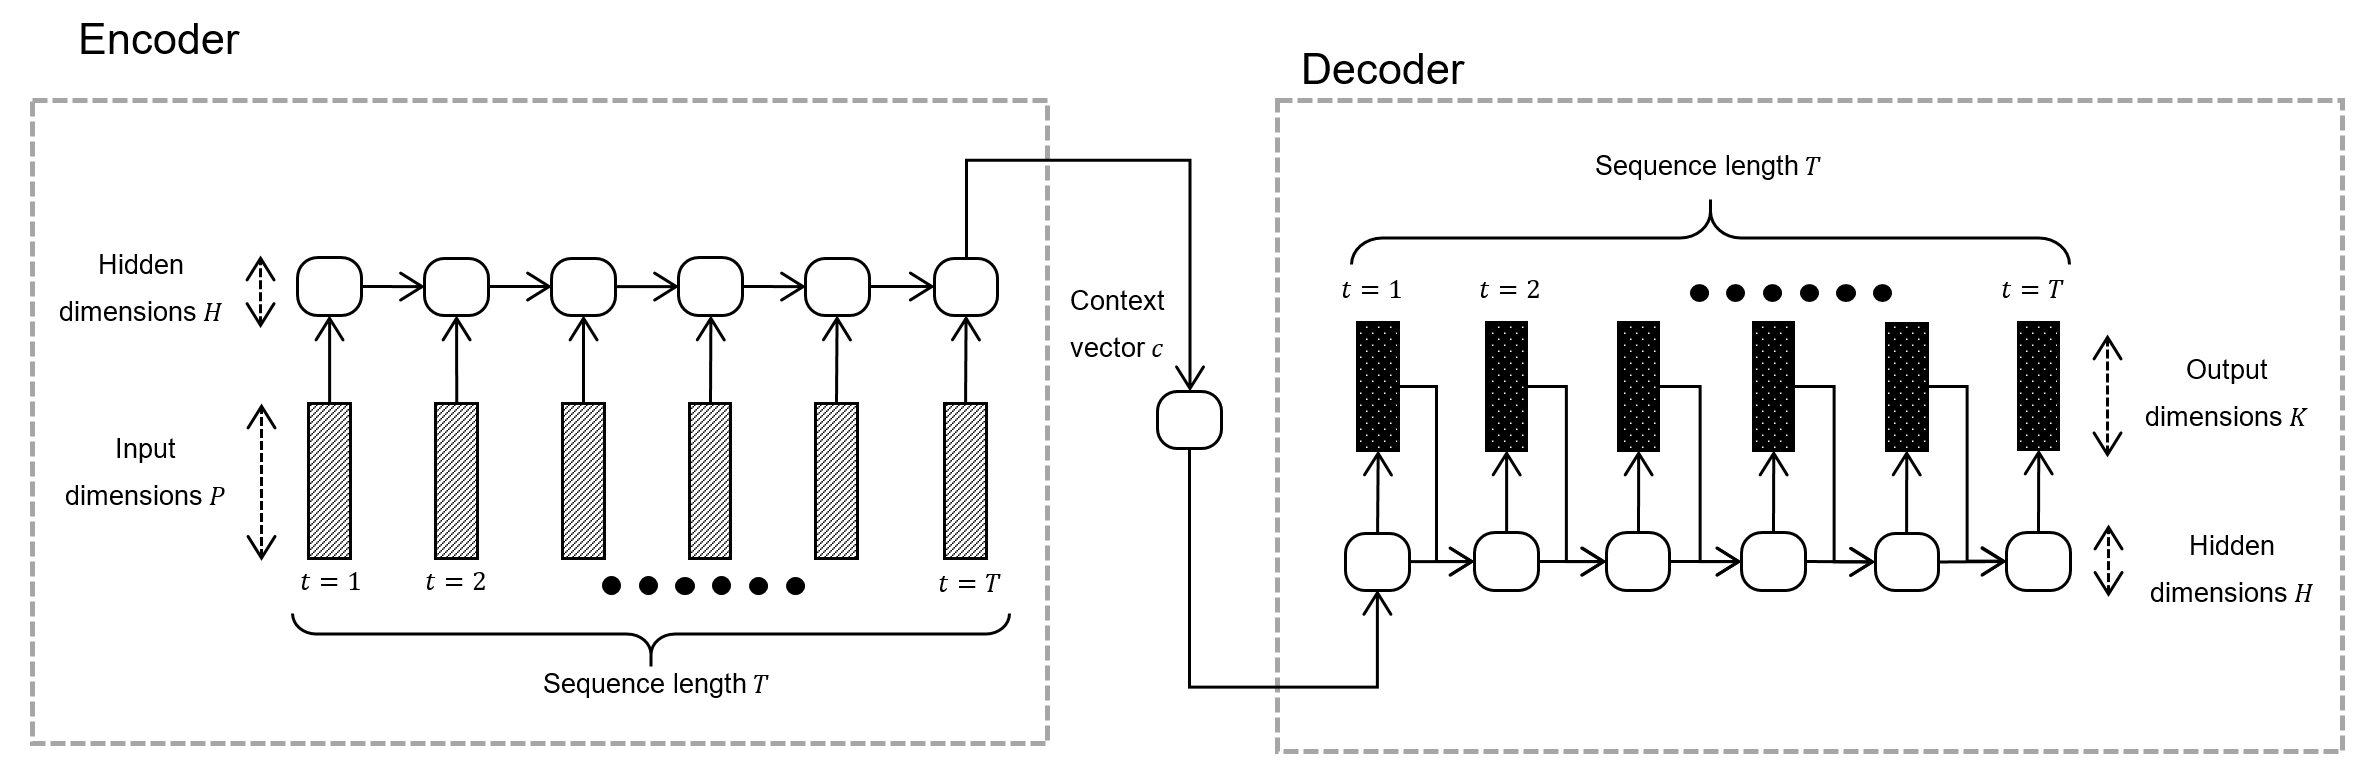
\includegraphics[width=0.8\textwidth]{seq2seq.PNG}
    \caption{RNN encoder-decoder model}
  \end{figure}
\end{frame}

\begin{frame}{Long-short term memory}
LSTM neuron \cite{hochreiter1997}
  \begin{figure}[H]
  	\centering
  	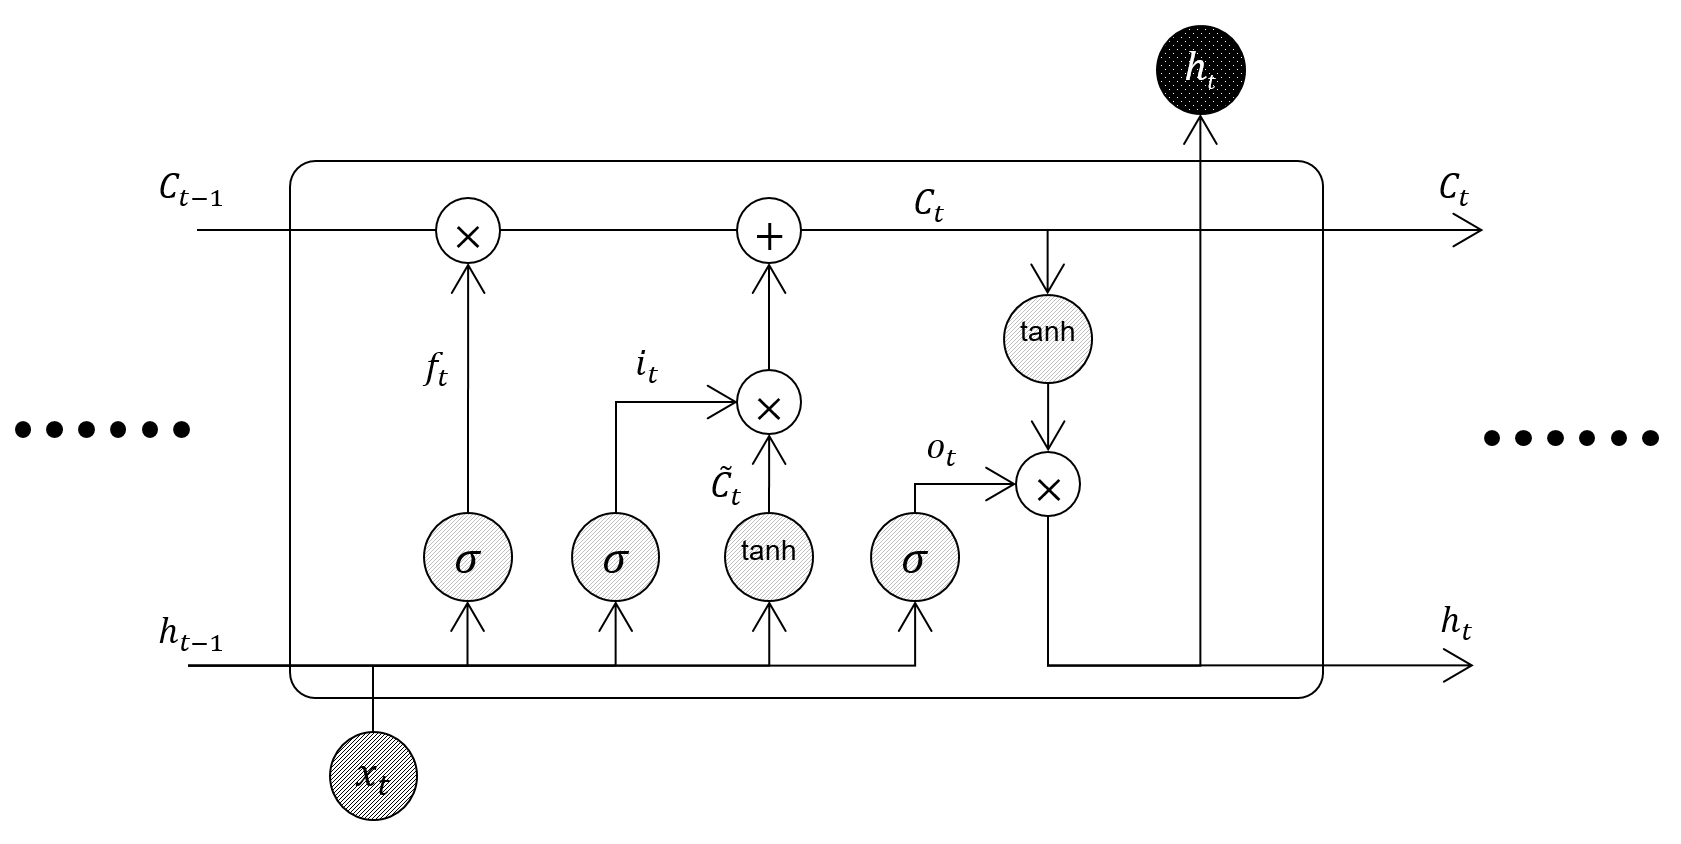
\includegraphics[width=1\textwidth]{lstm.PNG}
  	\caption{Internal structure of a long short-term memory block \cite{olah}.}
  \end{figure}
\end{frame}

\begin{frame}{Long-short term memory}
  Forget gate
	\[	f_t=\sigma(W_f[h_{t-1},x_t]+b_f) \]
	Input gate
	\[ i_t=\sigma(W_i[h_{t-1},x_t]+b_i) \]
	\[ \tilde{C}_t=\tanh (W_c[h_{t-1},x_t]+b_C) \]
	Update hidden state
	\[ C_t=f_t\times C_{t-1}+i_t\times\tilde{C}_t \]
	Output gate
	\[ O_t=\sigma(W_o[h_{t-1},x_t]+b_o) \]
	\[ h_t=O_t\times\tanh C_t \]
\end{frame}

\begin{frame}{Regularisation}
\begin{columns}[T] % align columns
\begin{column}{.58\textwidth}
\begin{itemize}
  \item Prevents network overfitting
  \item Dropout wrapper \cite{srivastava2014}
  \item Masks neuron inputs
  \item Non-recurrent connections only \cite{zaremba2014}
\end{itemize}
\end{column}%
\hfill%
\begin{column}{.38\textwidth}
\begin{figure}[H]
	\centering
	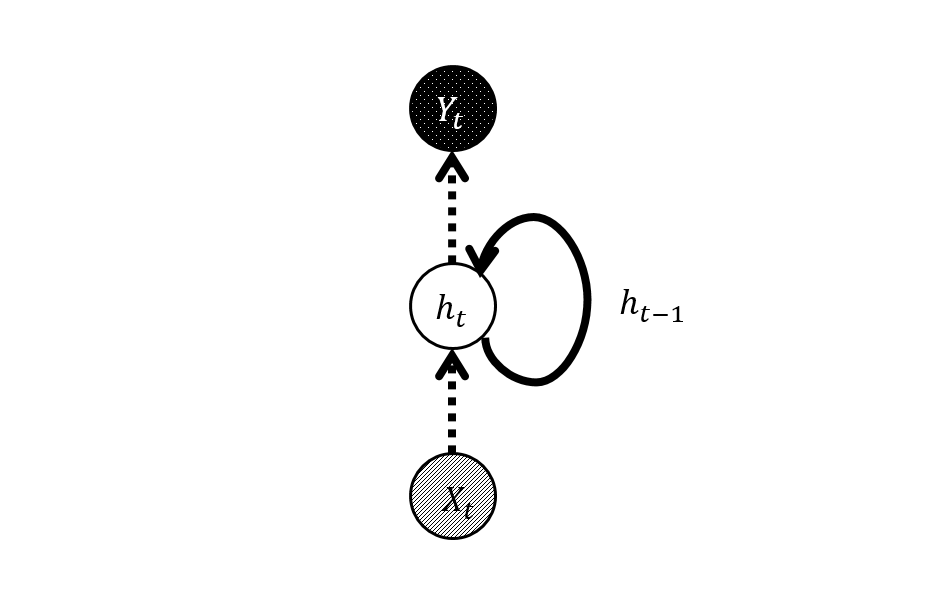
\includegraphics[width=1\textwidth]{dropout.PNG}
\end{figure}
\end{column}%
\end{columns}
\end{frame}

\begin{frame}{Sampling}
  \begin{itemize}
    \item Recursively generating time series samples with fixed length
    \item Samples of length \(T\) can be generated from any time series dataset with length \(T^{'} \geq T \)
    \item \(T^{'}-T\) samples can be generated
  \end{itemize}
  
  
  \begin{algorithm}[H]
  	\label{consecutive_sampling}
  	\caption{Drawing samples consecutively from the original dataset}
  	\SetKwInOut{Input}{Input}
  	\Input{Dataset length \(T^\prime\)}
  	\Input{Sample length \(T\)}
  	\(i\leftarrow 0\) \;
  	\While{\(i \leqslant i+T \) } {
  		Generate sample sequence \((i, i+T]\) from the dataset\;
  		\(i\leftarrow i+1\)\;
  	}
  \end{algorithm}
\end{frame}

\begin{frame}{Scaling}
  \begin{itemize}
    \item Standardising dataset using \(z\)-score
  \end{itemize}
  \[ z_p=\frac{x_p-\bar{x}_p}{\sigma_p} \]
\end{frame}

\begin{frame}{Results}
  \begin{figure}[h]
  	\centering
  	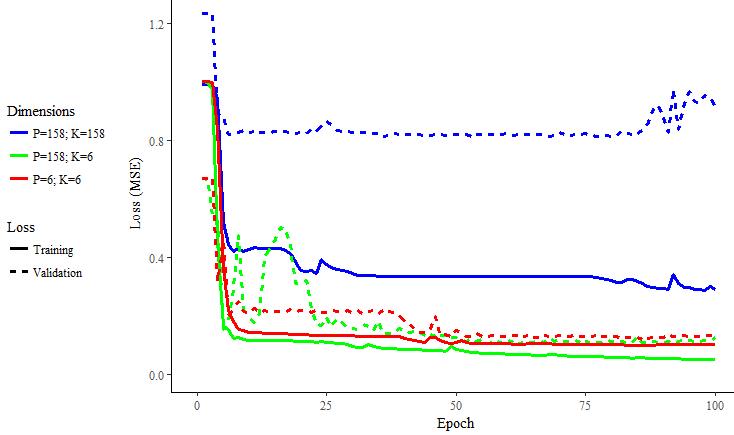
\includegraphics[width=0.65\textwidth]{output_dims.png}
  	\caption{Effects of relaxing dimensionality of the output sequence on the training and validation MSE losses.}

  \end{figure}
\end{frame}

\begin{frame}[shrink]{Sequence Reconstruction}
  \begin{itemize}
    \item Specimens were selected randomly for qualitative examination
    \item Selected from held-out validation set
  \end{itemize}
  \begin{figure}[H]
  	\centering
  	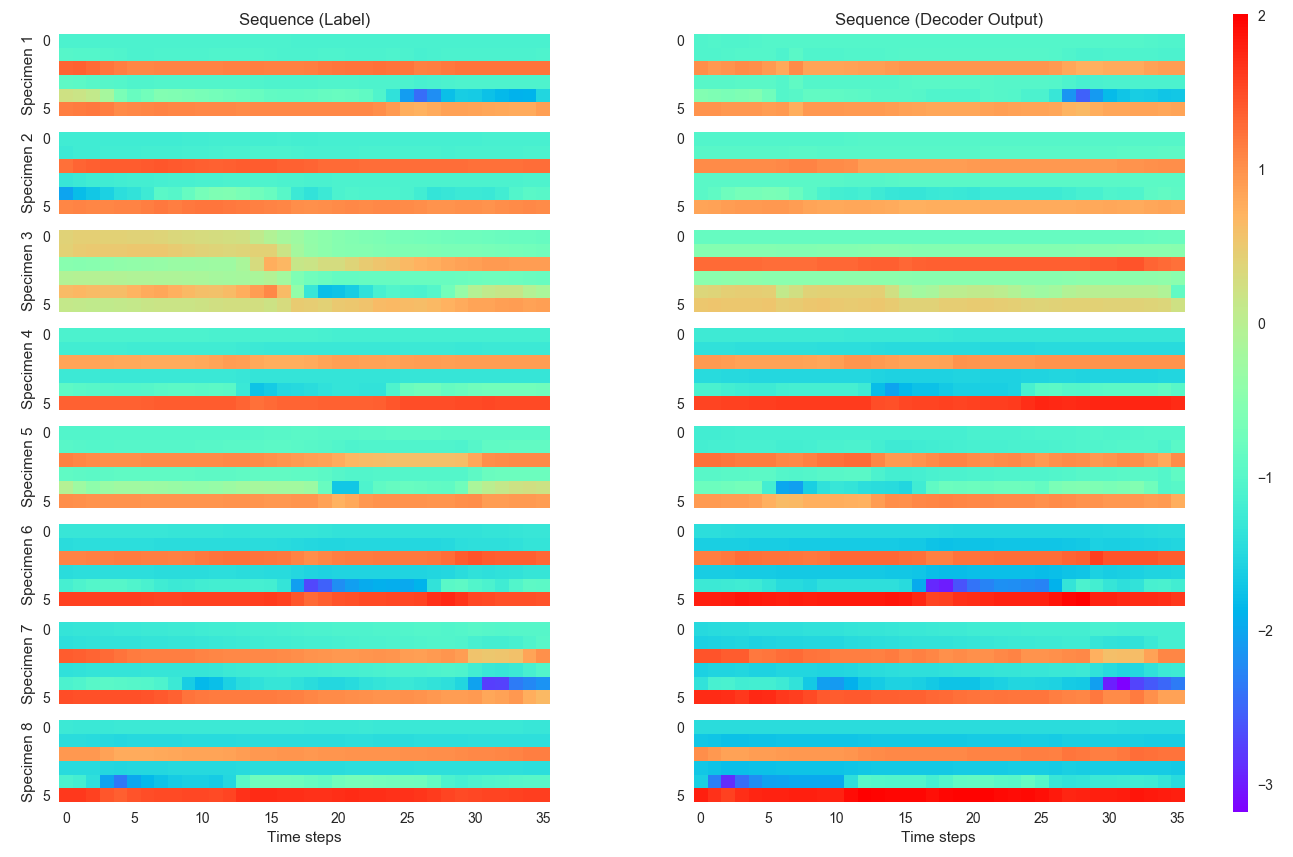
\includegraphics[width=1\textwidth]{heatmaps.png}
  	\caption{Randomly selected output sequences in the held-out validation set. Colour represents magnitude of sensor measurements in normalised scale.}
  \end{figure}
\end{frame}


\begin{frame}[shrink]{Context Vector}
  \begin{itemize}
    \item Pairwise Pearson correlation
    \item Diagonal shows strong correlation among successive context vectors
    \item Showing gradual drift of operating state
  \end{itemize}
  \begin{figure}[H]
  	\centering
  	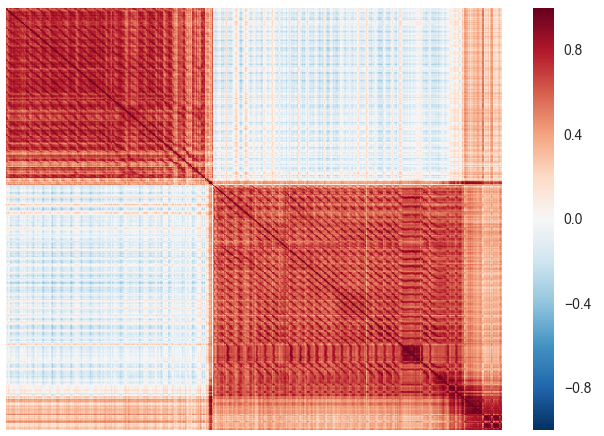
\includegraphics[width=1\textwidth]{matrix.PNG}
  \end{figure}
\end{frame}


\begin{frame}{Context Vector}
  \begin{itemize}
    \item Dimensionality reduction (PCA) to 2D
    \item Additional clustering algorithms can be applied (e.g. \(K\)-means)
    \item Decision boundary calculated using Support Vector Machine (RBF)
  \end{itemize}
\end{frame}


\begin{frame}[shrink]{Context Vector: Example 1}
\begin{figure}[H]
	\centering
	\begin{subfigure}[b]{0.5\textwidth}
		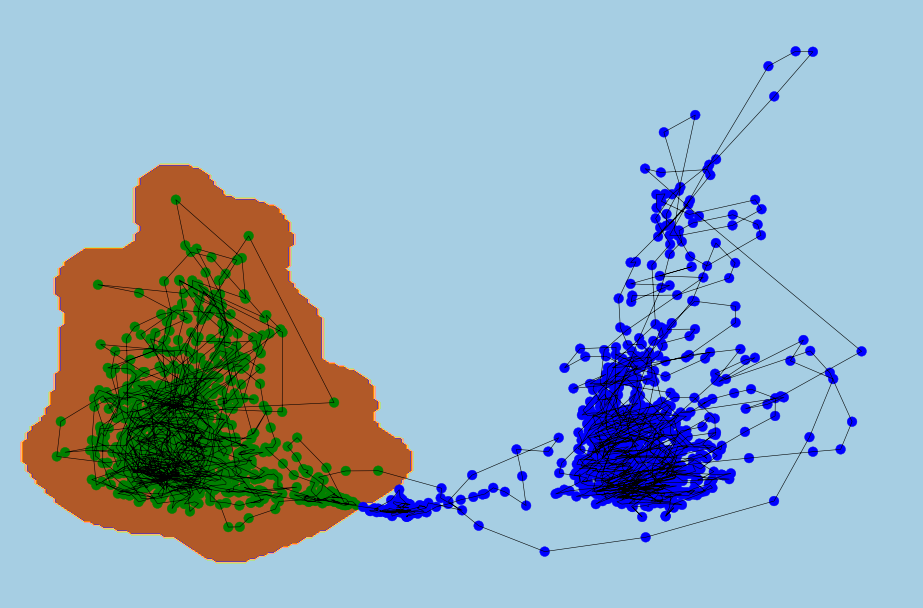
\includegraphics[width=\textwidth]{pca_cluster_2.png}
		\caption{\(2\) clusters}
		\label{fig:pca_cluster_2}
	\end{subfigure}
	~
	\begin{subfigure}[b]{0.25\textwidth}
		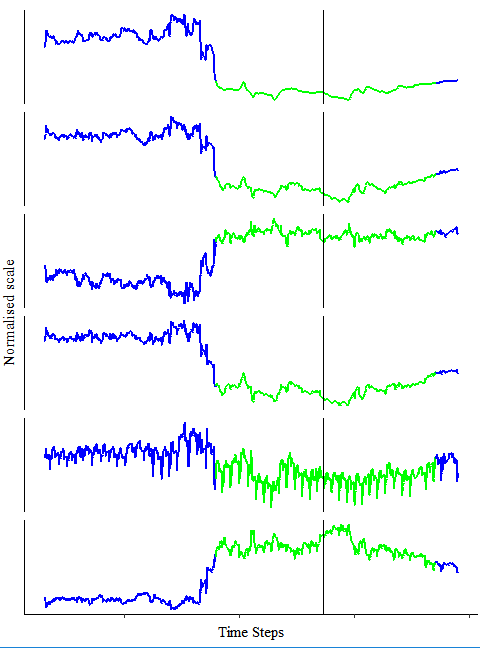
\includegraphics[width=\textwidth]{context_timeline_2.png}
		\label{fig:context_timeline_2}
	\end{subfigure}
	
	\begin{subfigure}[b]{0.5\textwidth}
		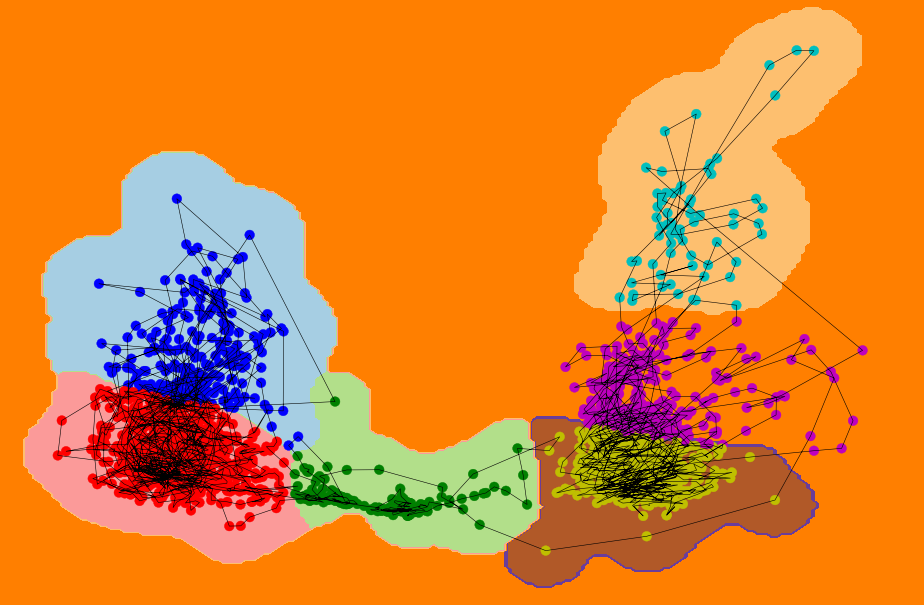
\includegraphics[width=\textwidth]{pca_cluster_6.png}
		\caption{\(6\) clusters}
		\label{fig:pca_cluster_6}
	\end{subfigure}
	~
	\begin{subfigure}[b]{0.25\textwidth}
		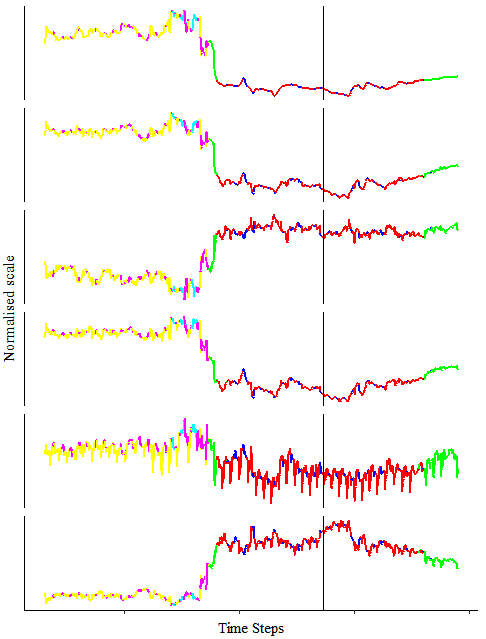
\includegraphics[width=\textwidth]{context_timeline_6.png}
		\label{fig:context_timeline_6}
	\end{subfigure}
	
\end{figure}
\end{frame}

\begin{frame}[shrink]{Context Vector: Example 2}
\begin{figure}[H]
	\centering
	\begin{subfigure}[b]{0.35\textwidth}
		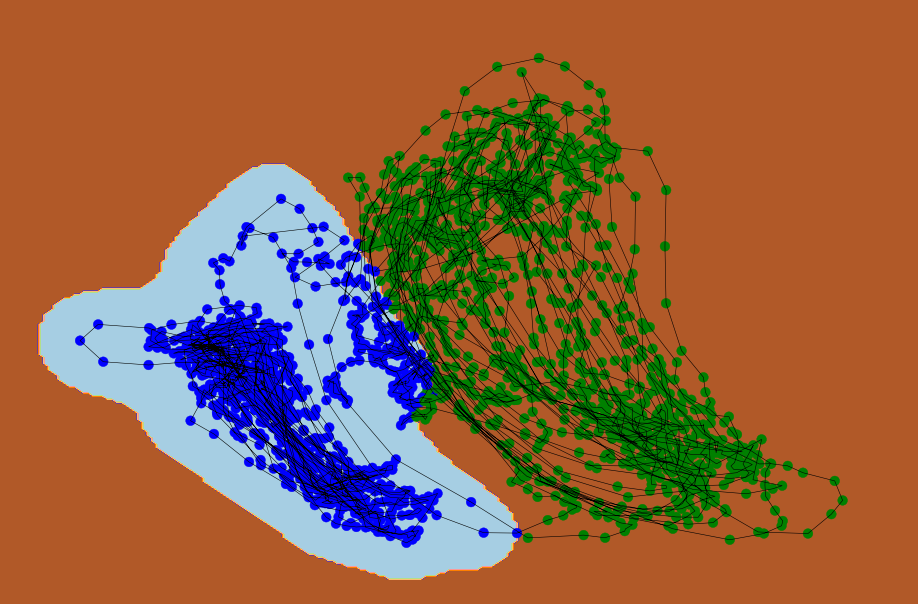
\includegraphics[width=\textwidth]{ex2_pca_cluster_2.png}
		\caption{\(2\) clusters}
		\label{fig:ex2_pca_cluster_2}
	\end{subfigure}
	~
	\begin{subfigure}[b]{0.6\textwidth}
		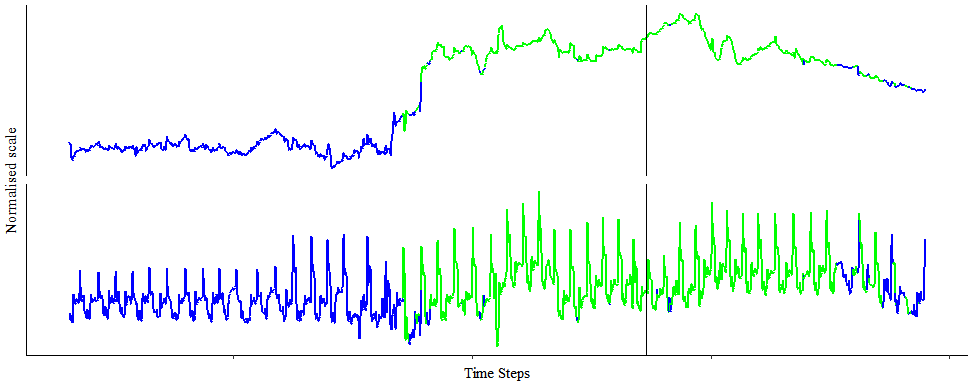
\includegraphics[width=\textwidth]{ex2_context_timeline_2.png}
		\label{fig:ex2_context_timeline_2}
	\end{subfigure}
	
	\begin{subfigure}[b]{0.35\textwidth}
		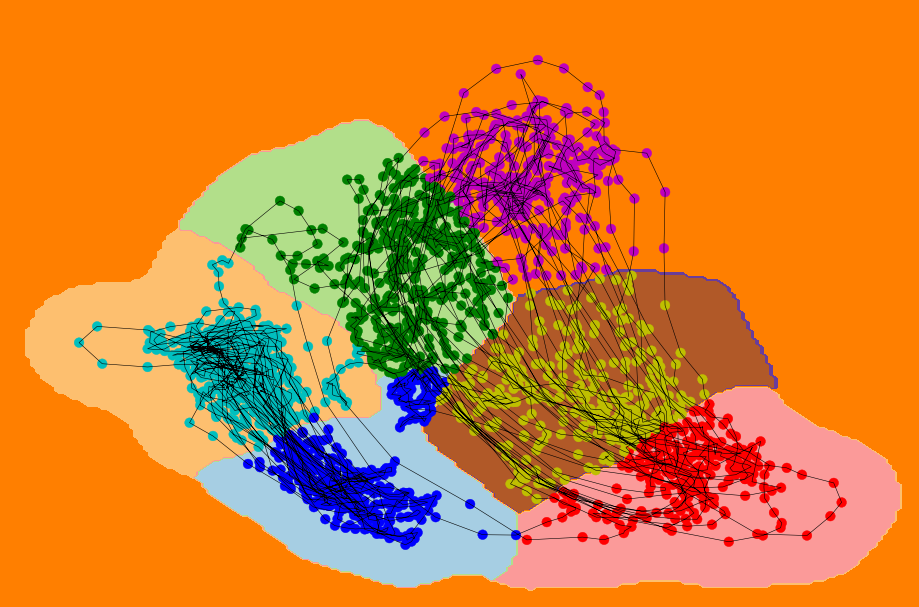
\includegraphics[width=\textwidth]{ex2_pca_cluster_6.png}
		\caption{\(6\) clusters}
		\label{fig:ex2_pca_cluster_6}
	\end{subfigure}
	~
	\begin{subfigure}[b]{0.6\textwidth}
		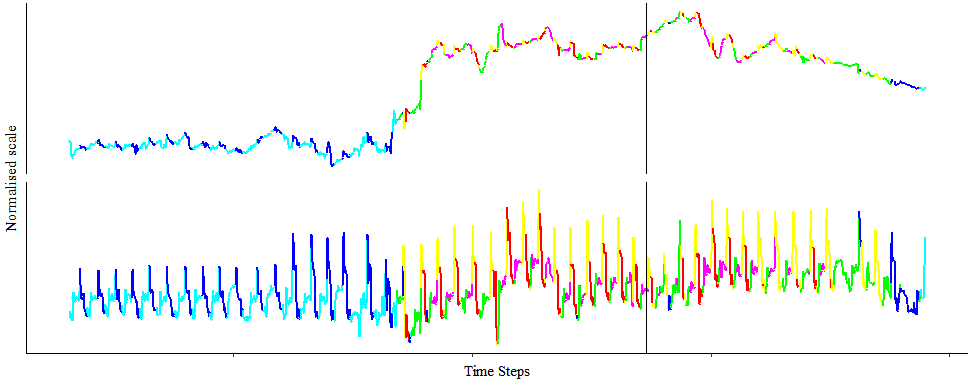
\includegraphics[width=\textwidth]{ex2_context_timeline_6.png}
		\label{fig:ex2_context_timeline_6}
	\end{subfigure}
\end{figure}

\end{frame}

\begin{frame}[shrink]{Identify Operating States}
  \begin{enumerate}
    \item Drifts around same neighbourhood
    \item Drifts across boundary
  \end{enumerate}
\begin{figure}[H]
	\centering
	\begin{subfigure}[b]{0.3\textwidth}
		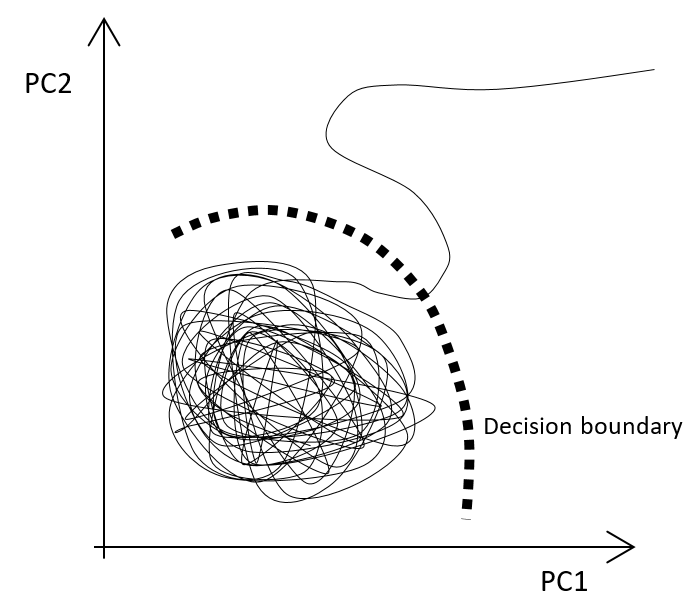
\includegraphics[width=\textwidth]{contexttravel.PNG}
		\caption{Process with a single healthy state.}
		\label{fig:contexttravel}
	\end{subfigure}
	~
	\begin{subfigure}[b]{0.3\textwidth}
		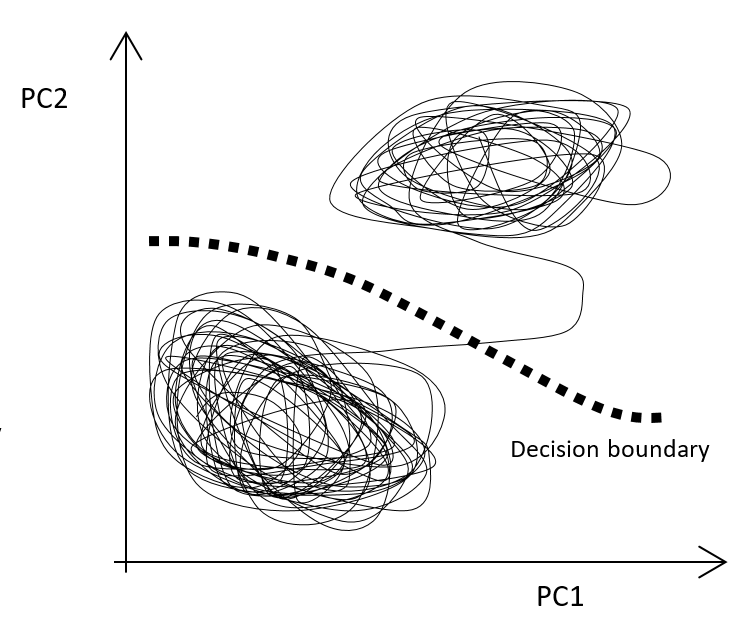
\includegraphics[width=\textwidth]{contexttravel2.PNG}
		\caption{Multi-state process with transition between states.}
		\label{fig:contexttravel2}
	\end{subfigure}
	\caption{Travelling context vector.}
\end{figure}
\end{frame}



\begin{frame}{Input Sequence Reversal}
  \begin{itemize}
    \item Forward sequence: \(\{\mathbb{R}_1^P, \mathbb{R}_1^P, \mathbb{R}_3^P,...,\mathbb{R}_{T-1}^P, \mathbb{R}_T^P \}\)
    \item Reverse sequence: \(\{\mathbb{R}_T^P, \mathbb{R}_{T-1}^P, \mathbb{R}_{T-2}^P,...,\mathbb{R}_2^P, \mathbb{R}_1^P \}\)
  \end{itemize}
  \begin{figure}[H]
  	\centering
  	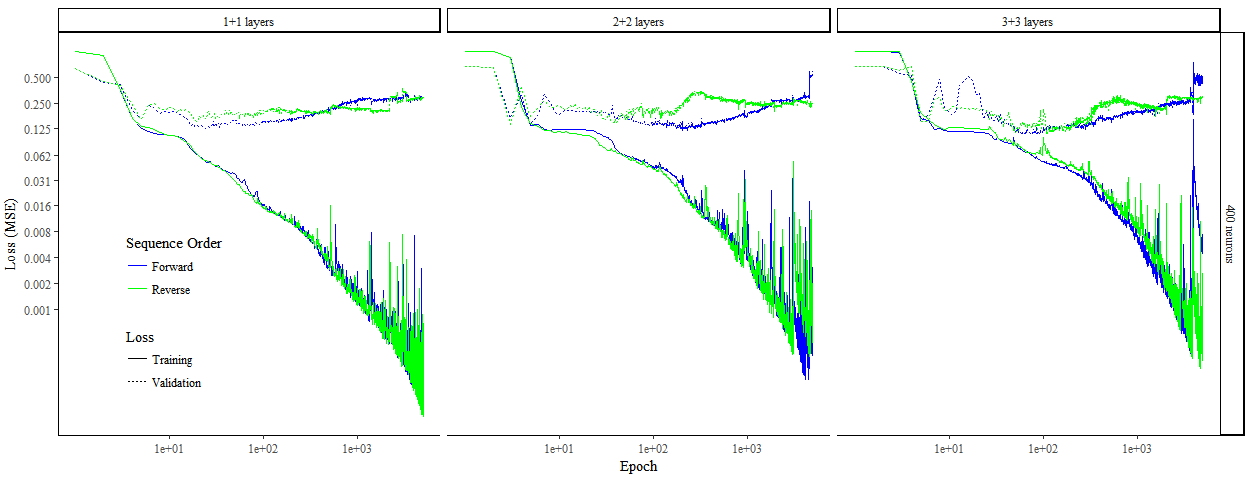
\includegraphics[width=1\textwidth]{reverse.PNG}
  	\caption{Effects of sequence reversal on training/validation MSE losses.}
  \end{figure}
\end{frame}



\begin{frame}{Adjusting Sequence Length}
  \begin{itemize}
    \item Training/validation loss goes up when sequednce length \(T\) is increased.
  \end{itemize}
  \begin{figure}[H]
  	\centering
  	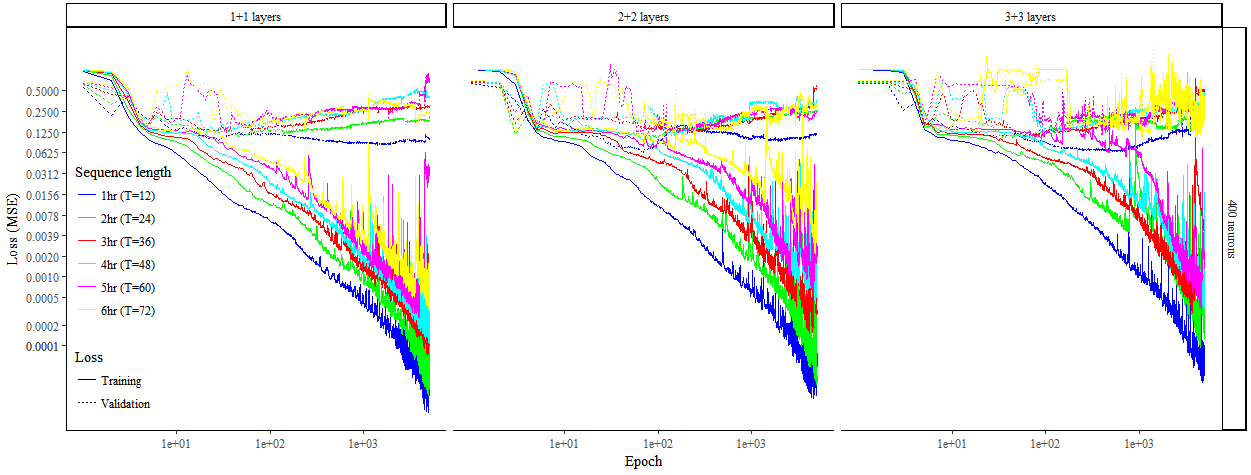
\includegraphics[width=1\textwidth]{sequence_length.PNG}
  	\caption{Effects of sequence length on training/validation MSE losses.}
  \end{figure}
\end{frame}





\begin{frame}[shrink]{Summary}
  \begin{itemize}
    \item Unsupervised clustering method for multidimensional time series
    \item Neural network-based time series feature selection
    \item Works with any real-  valued temporal measurement (e.g. temperature, pressure… etc.)
    \item Operating states identification
  \end{itemize}
\end{frame}

\begin{frame}[allowframebreaks]{Bibilography}
  \bibliographystyle{amsalpha}
  \bibliography{mybibliography}
\end{frame}

\end{document}